\chapter{The big reform agenda: creating an adaptive education system design}\label{chap:Design_an_adaptive_system_of_continuous_improvement}

This chapter discusses how to achieve a system of continuous school improvement, and the broader system settings needed to help teachers to know what works best for their students and how they can translate this into daily classroom practice. 

A top-down model is not sufficient for sustained improvement. But neither is a bottom-up system, with 10,000 schools doing their own thing. 

A strong evidence base on `what works' is just the beginning: many other factors also need to be in place for teachers to embed evidence in their classroom practice. A more `adaptive' system design is needed, with stronger feedback loops for more systematic learning.

\section{Create a more adaptive education system}\label{sec:Create-a-more-adaptive-education-system}

School education in Australia faces three big challenges: 

\begin{itemize}
    \item First, we must improve the teaching of core foundational skills, where the challenge is largely about how to spread what works best. 
    \item Second, we need to better prepare young people in `new' capabilities in critical thinking and non-cognitive capabilities, where we know little about what works best.
    \item Third, we must address the large gaps between advantaged and disadvantaged groups.
\end{itemize}

The system must be designed to cater to each of these very different challenges. It needs to encourage teachers to embed clear, existing evidence where it exists (for example on core foundational skills), and at the same time enable disciplined innovation where the evidence is weak (for example in critical thinking and non-cognitive skills). An adaptive education system gives adequate direction to teachers, but also ensures they are equipped to make sound judgments where there is ambiguity.%
\footnote{For further discussion see the Grattan Institute report, Towards an adaptive education system in Australia (\textcite{Goss2017TowardsAnAdaptiveSystem}).}

Adaptive improvement is best thought of as an iterative, deliberate way to learn by doing, using a feedback loop with an explicit focus on inputs and outcomes as well as the learning processes along the way. Adaptive reform uses data to link what is done (inputs) to what is learnt (outcomes) and systematically improve the learning process over time. An adaptive system ensures that all parts of the system promote learning.


\begin{figure}
\caption{The Grattan Institute model shows how to use feedback loops to improve education outcomes\label{fig:Grattan-Institute-Model}}
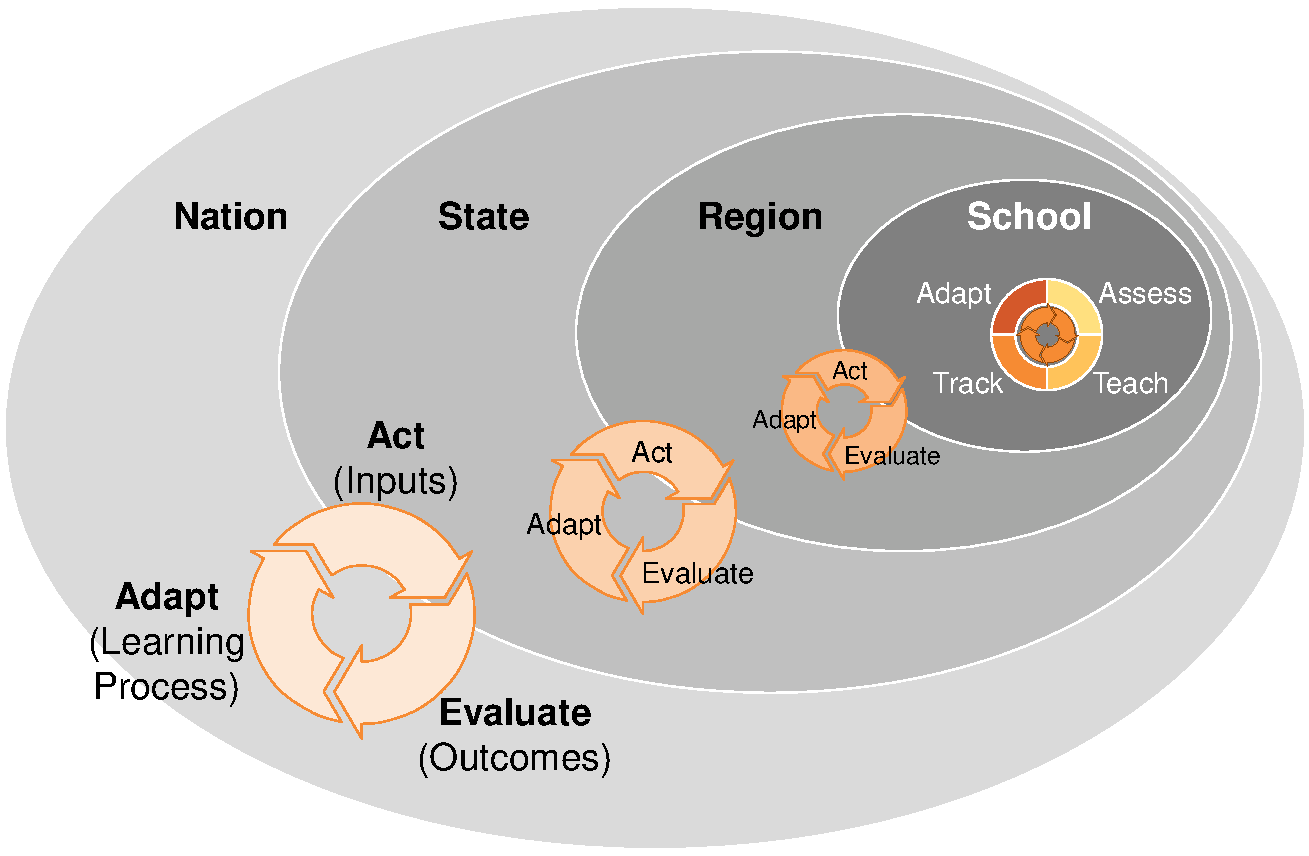
\includegraphics[page=1]{charts/GonskiReportCharts.pdf}
\source{\textcite{Goss2017TowardsAnAdaptiveSystem}
Note the school level feedback loop of `assess, teach, track and adapt' embeds the idea of targeted teaching which is at the heart of adaptive improvement.}
\end{figure}



\section{Strengthen feedback loops at multiple levels}\label{sec:Strengthen-feedback-loops-at-multiple-levels}

School education has been much slower than other professions such as medicine and engineering to produce scientific evidence and incorporate it into practice. Even where the evidence is clear, it is not necessarily taken up. This is not only an issue in schools, but also in government policy making.  

An adaptive education system has strong evaluative structures and feedback loops to help embed evidence in practice. \Vref{fig:Grattan-Institute-Model} depicts such a system, with feedback loops at four levels: school, region, state, and nation. 

At a minimum there are three steps in any feedback loop: (i) `Act' by deliberately selecting inputs or programs to meet needs; (ii) `Evaluate' by tracking and measuring the outcomes; and (iii) `Adapt' by using learnings on what worked best to inform actions next time around.

Feedback mechanisms can encourage a more evaluative way of working, but a range of other barriers to using evidence need to be overcome too. The next sections discuss some of those barriers.




\begin{figure}
\caption{There are many possible reasons people do not use evidence in practice\label{fig:There-are-many-possible-reasons-people-do-not-use-evidence-in-practice}}
\includegraphics[page=2]{charts/GonskiReportCharts.pdf}
\source{Adapted from \textcite{ProductivityCommission2016NationalEvidenceBase}}
\end{figure}


\section{Better understand why people use evidence (or don’t)}\label{sec:Better-understand-why-people}

%ERROR
There are many possible reasons schools and policy makers do not use evidence in daily decisions, as shown in \Vref{fig:There-are-many-possible-reasons-people-do-not-use-evidence-in-practice}.
%
Research findings need to be readily accessible, timely, relevant and trustworthy. The organisational culture must support risk-taking. Individuals must possess the skills to translate and implement the evidence. Interaction between researchers and public servants can be beneficial, including at the departmental level.



\subsection{System-level policies can increase the uptake of evidence}\label{subsec:System-level-policies-can-increase-the-uptake-of-evidence}

Government policies can increase the use of evidence in daily decisions, but there is little high-quality research on exactly what system policies and programs are most effective. 

Studying high-performing education systems can shed some light on the types of policies likely to help in spreading evidence. Some OECD research points to a mix of policies for system-wide improvement and behaviour change in schools, including both vertical and horizontal accountability, as well as capacity building initiatives.%
\footcite{BurnsKoster2016GoverningEducation}

School education literature includes some research on the conditions that facilitate `adult learning' and improvement, but more is needed.\footnote{For a summary of the research on how adults `learn' professionally, see \textcite{Jensen2016PDTeacherProfessional}.}
One common theme is that collaboration and professional learning communities can play a big role in shifting attitudes (when done well), because it encourages deep conversations among practitioners that can challenge existing beliefs over time. Other qualitative literature suggests school improvement is not so much about changing mindsets as changing behaviours.\footcite{Macklin2017DrivingSchoolImprovement}
It suggests routines can be a powerful tool to get teachers to change behaviour. They first experience the benefits for student learning, which then influences a shift in mindset later on. The Productivity Commission has identified this as an issue for further research in Australia.\footcite{ProductivityCommission2016NationalEvidenceBase}

`Improvement' science can help shed light on what school settings are needed to translate evidence into practice. It involves researchers working directly with educators to adapt evidence to local needs and solve specific problems of practice. This collaborative structure can help persuade sceptical educators that scientific research is relevant to their specific context.

But improvement science is not a system-wide solution; large-scale improvement will only come with better-designed experiments that also incorporate steps on how to actually implement the practice under investigation, including the guidance or system supports needed.%
  \footcite{Dynarski2015UsingresearchtoimproveeducationundertheEveryStudentSucceedsAct}
This is the focus of the growing field of implementation science research.%
  \footnote{Implementation science is slightly different to improvement science; it studies the methods and approaches to help update and integrate research findings into routine practice.}

The Gonski 2.0 Review team should synthesise the existing research on how best to implement what works. It should explore research in:

\begin{itemize}
    \item Literature from school education, psychology, public policy, management, organisational change, improvement science and implementation science. 
    \item System design in high-performing school education systems, including the system-level policies and programs for spreading evidence-based practice.\footcite{Jensen2012CatchingUpLearning}
    \item Other professional sectors, including nursing, medicine, engineering and aviation.
\end{itemize}

Such research will be useful for schools, but also for policy makers in designing the system-level policies and structures most likely to improve classroom teaching. 

The next chapter identifies more specific system-level reforms that can help build a more adaptive education system. 


